\documentclass[aspectratio=169]{beamer}
% далее идёт преамбула
%\usepackage{xltxtra}
\usepackage[utf8]{inputenc}
\usepackage[main=russian,english]{babel}
\usepackage{moreverb}
\usepackage{graphicx}

\title{Сравнительный анализ библиотек глубокого обучения}
\author{Козенко~В.~С.}

%\setmainfont{Arial}

\begin{document}% начало презентации

\begin{frame}
\titlepage
\end{frame}

\begin{frame}{Цель}
	В 21 веке глубокое обучение, и машинное обучение в целом, очень активно развивались, в следствии чего возникло множество библиотек глубокого обучения, и непосвященному разработчику доставляет трудность выбор подходящей для его задачи библиотеки обучения. Данная работа ставит своей целью помощь таким разработчикам и осуществляет сравнение наиболее популярных на данный момент библиотек.
\end{frame}

\begin{frame}{Этапы работы}
	\begin{enumerate}
		\item Поерхностное сравнение библиотек TensorFlow, Keras, PyTorch;
		\item Разделение всех библиотек на глобальные семейства;
		\item Практическое сравнение библиотек TensorFlow, Keras, PyTorch;
		\item Написание этой презентации.
	\end{enumerate}	
\end{frame}

\begin{frame}{Введение}
Сейчас существует множество библиотек глубокого обучения. Мы сравним три самых популярных и широкоиспользуемых библиотек: 
\begin{itemize}
	\item[$-$]TensorFlow;
	\item[$-$]Keras;
	\item[$-$]PyTorch.
\end{itemize}
\end{frame}

\begin{frame}{Немного о самих библиотеках}
\begin{itemize}
\item[$\bullet$] TensorFlow - открытая библиотека для машинного обучения, разработанная компанией Google, для решения задач построения и тренировки нейронных сетей. Основной API для работы с библиотекой реализован для Python.

\item[$\bullet$] PyTorch - библиотека машинного обучения для языка Python с открытым исходным кодом, созданная на базе Torch. Разрабатывается преимущественно группой искусственного интеллекта Facebook.

\item[$\bullet$] Keras - открытая нейросетевая библиотека, написанная на языке Python. Она представляет собой надстройку над фреймворками Deeplearning4j, TensorFlow и Theano. Нацелена на оперативную работу с сетями глубинного обучения, при этом спроектирована так, чтобы быть компактной, модульной и расширяемой.
\end{itemize}
\end{frame}

\begin{frame}{О семействах современных библиотек глубокого обучения}
Все современные библиотеки глубокого обучения можно глобально разделить на три группы:
\begin{itemize}
\item[$\bullet$] Фреймворки с фиксированные модулями.

В таких фреймворках пользователь комбинирует уже готовые блоки в граф вычислений и запускает его. Прямой и обратный проход уже предусмотрен в каждом блоке. Расширяемость близка к нулю: определять новые блоки гораздо сложнее, чем использовать уже готовые. Однако, если готовых блоков достаточно для вашей задачи, то скорость разработки максимальна, как и скорость работы программы (т.к. заранее написанный код высоко оптимизирован). Такие библиотеки используются для прототипирования. К ним относится Keras, а так же Caffe, Caffe2, CNTK, Kaldi, DL4J.\end{itemize}
\end{frame}

\begin{frame}
\begin{itemize}
\item[$\bullet$] Фреймворки со статическим графом вычислений.

С помощью таких фреймворков уже можно создавать вычислительные графы произвольной сложности и размера, однако, после компиляции, в нем ничего изменить нельзя будет: он будет доступен только для прямого и обратного проходов. Из-за этого возрастает сложность отладки программы. Все такие фреймворки используют декларативный стиль программирования и напоминают функциональный язык или математическую нотацию. Представителями этого класса являются TensorFlow, а так же Theano, MXNet.
\end{itemize}
\end{frame}

\begin{frame}
\begin{itemize}
\item[$\bullet$] Фреймворки с динамическим графом вычислений.

В фреймворках данного класса граф вычислений строится при каждом запуске программы, при каждом проходе по нему, в отличии от предыдущего класса. Подобный подход даёт максимальную гибкость и расширяемость, позволяет использовать в вычислениях все возможности используемого языка программирования и не ограничивает пользователя вообще ничем. К этому классу фреймворков относятся Torch, PyTorch, Chainer, DyNet.
\end{itemize}

В нашем сравнении мы взяли по одному яркому представителю каждого из семейств.
\end{frame}

\begin{frame}{Сравнение синтаксиса на простейших примерах.}
	Сравнение реализации цикла \verb"while" на TensorFlow и на PyTorch.
	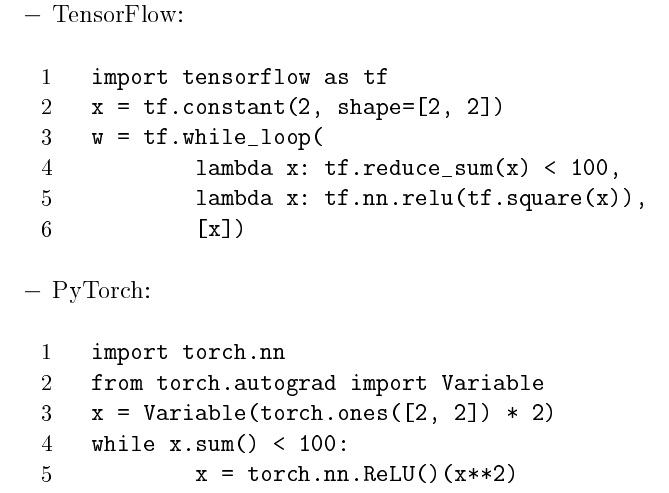
\includegraphics[width=200pt]{code.png}

\end{frame}

\begin{frame}{Выводы}
Связав все предыдущие параметры воедино, а так же заметив, что API TensorFlow предоставляет лишь простейшие инструкции по сборке, необходимые для создания расчетных графов, он лишен «стандартной библиотеки» для наиболее распространенных фрагментов программ. Поэтому более высокоуровневые API поверх TensorFlow реализованы сообществом, из-за чего их появилось множество и они совершенно различны (наиболее популярные из этих API: Keras, TFLearn, PrettyTensor, TF-Slim). В случае с PyTorch все сложилось иначе: он уже оснащен самыми ходовыми элементами, нужными для ежедневных исследований в области глубокого обучения. В PyTorch есть нативный Keras-подобный API в пакете torch.nn.
\end{frame}

\begin{frame}
\begin{tabular}[t]{| p{52pt} | p{65pt} | p{57pt} | p{54pt} | p{50pt} | p{50pt} |}
	\multicolumn{6}{r}{Таблица 1. 1.}\\
	\hline
	& \bf{Тип графа} & \bf{Логичность} & \bf{Поддержка новых операций} & \bf{Качество документации} & \bf{Удобность API} \\
	\hline
	\bf{PyTorch} & Динамический & Высокая & Python, C++ &  Высокое & Выслокая\\
	\hline
	\bf{TensorFlow} & Статический & Средняя & С++ & Среднее & Средняя\\
	\hline
	\bf{Keras} & Зависит от backend & Высокая & Python & Высокое & Средняя\\
	\hline
\end{tabular}
\end{frame}

\end{document}